\documentclass[hyperref={colorlinks = true},unknownkeysallowed]{beamer}
\usepackage{hyperref}%
\usepackage{graphicx} % graphics
\usepackage{epsfig} % eps graphics
\usepackage{booktabs, caption} % table styling
\usepackage{pgfplots}
\usepackage{amsmath}
\usepackage{tikz}
\usetikzlibrary{positioning}
\usetikzlibrary{fit}
\usetikzlibrary{backgrounds}
\usetikzlibrary{calc}
\usetikzlibrary{shapes}
\usetikzlibrary{mindmap}
\usetikzlibrary{decorations.text}
\usetikzlibrary{arrows.meta,arrows}
\usetikzlibrary{shapes.geometric}
\usepackage{changepage}
\usepackage{color}
\usepackage{caption}
\usepackage{transparent}
\usepackage{fontspec}
\usepackage{tcolorbox}
\usetikzlibrary{shapes}
\usepackage{natbib}
\bibliographystyle{plainnat}
\pgfplotsset{compat=1.7}

\makeatletter
\def\blfootnote{\xdef\@thefnmark{}\@footnotetext}
\makeatother

\definecolor{UBCblue}{rgb}{0.04706, 0.13725, 0.26667} % UBC Blue (primary)
\usecolortheme[named=UBCblue]{structure}

\let\oldbibitem=\bibitem
\renewcommand{\bibitem}[2][]{\label{#2}\oldbibitem[#1]{#2}}
\let\oldcite=\cite
\renewcommand\cite[1]{\hypersetup{linkcolor=UBCblue} \hyperlink{#1}{\oldcite{#1}}}
\let\oldcitep=\citep
\renewcommand\citep[1]{\hypersetup{linkcolor=UBCblue}\hyperlink{#1}{\oldcitep{#1}}}
\let\oldciteauthor=\citeauthor
\renewcommand\citeauthor[1]{\hypersetup{linkcolor=UBCblue}\hyperlink{#1}{\oldciteauthor{#1}}} 


% suppress navigation bar
\beamertemplatenavigationsymbolsempty

\setbeamercolor{normal text}{fg=UBCblue}
\setbeamercolor{frametitle}{bg=white, fg=UBCblue}

\setbeamercolor{section title}{fg=UBCblue, bg=white}
\setbeamercolor{headline}{bg=white, fg=UBCblue}
\setbeamercolor*{palette primary}{fg=UBCblue,bg=UBCblue}
\setbeamercolor*{palette secondary}{fg=UBCblue,bg=UBCblue}
\setbeamercolor*{palette tertiary}{fg=UBCblue,bg=UBCblue}

\setbeamertemplate{itemize subitem}[triangle]


% see the macros.tex file for definitions
\include{macros}

% command shortcuts
\newcommand{\tikzmark}[1]{\tikz[overlay,remember picture] \node (#1) {};}
\tikzset{
	block/.style={rectangle, draw, fill=white!40, text width=13em,
		text centered, rounded corners, minimum height=2em},
}
\newcommand{\thinkB}[1] {
	\begin{tikzpicture}
	\node [rectangle, draw, decoration=bumps, decorate, align=left, inner sep=4mm] {#1};
	\end{tikzpicture}
}

\newcommand{\thinkA}[1] {
	\begin{tikzpicture}
	\node[cloud, draw, align=left, cloud puffs=20,cloud puff arc=110, aspect=2, minimum width=.3cm, minimum height=.3cm, inner sep=0pt,
	text width=6.5cm, inner sep=0mm]{#1};
	\end{tikzpicture}
}


% for resuming lists across frames
\newcounter{savedenum}
\newcommand*{\saveenum}{\setcounter{savedenum}{\theenumi}}
\newcommand*{\resume}{\setcounter{enumi}{\thesavedenum}}

\setbeamertemplate{bibliography entry article}{}
\setbeamertemplate{bibliography entry title}{}
\setbeamertemplate{bibliography entry location}{}
\setbeamertemplate{bibliography entry note}{}


% title slide definition
\title{Data Summarizations for Scalable, Robust and Privacy-Aware Learning in High-Dimensions}
\author{Dionysis Manousakas}
\institute{Department of Computer Science \& Technology, \\University of Cambridge}
\date{}

%--------------------------------------------------------------------
%                           Introduction
%--------------------------------------------------------------------

\begin{document}
	
\begin{frame}
\vspace{2cm}
  \titlepage
  \vspace{10cm}
\end{frame}

\begin{frame}{Structure}
	\begin{itemize}
		\item[I.]\textbf{Quantifying Privacy Loss of Human Mobility Graph Topology}  \small{\citep{manousakas2018quantifying}} \\
		An empirical study on longitudinal mobility data, highlighting overlooked privacy threats on reduced data representations
		\item[II.]\textbf{Bayesian Pseudocoresets} \small{\citep{psvi}} \\
		A variational framework for scalable Bayesian inference, that achieves superior summarization quality in high-dimensions and admits differentially private constructions
		\item[III.]\textbf{$\beta$-Cores} \small{\citep{beta-cores}}  \\
		A framework for Bayesian summarization designed for observations following the Huber contamination model.
	\end{itemize}
\end{frame}

\begin{frame}
	\LARGE{\textbf{I. Quantifying Privacy Loss of Human Mobility Graph Topology}}
\end{frame}

\begin{frame}{ Mobility data privacy vs. utility}
	\vspace*{2.25mm}
\begin{block}{ $\bullet$ Information sharing for data-driven customization and large-scale analytics}
	\begin{itemize}
		  \setlength\itemsep{.3em}
		\item --- context-awareness
		\item --- transportation management, health studies, urban development
	\end{itemize}
\end{block}
%\pause
\begin{block}{ $\bullet$ \textbf{Utility}-preserving anonymized data representations}
	\begin{itemize}
		  \setlength\itemsep{.3em}
	%\item timestamped GPS measurements
	\item --- histograms, heatmaps, \textbf{graphs}
	\end{itemize}
\end{block}
%\pause
\begin{block}{ $\bullet$ How \textbf{privacy} conscientious they are?}
	\begin{itemize}
		\item --- often poorly understood, leading to privacy breaches
	\end{itemize}
\end{block}
\end{frame}


\begin{frame}{Deanonymizing mobility}
	%\includegraphics[width=5cm,height=3.5cm]{figs/rawtraces.png}
	\begin{columns}
		\begin{column}[t]{0.5\textwidth}
	\begin{block}{Inference on \textbf{individual}  traces }
	\circled{\textbf{1}} Sparsity and regularity-based \\
	\begin{itemize}
		\item --- "top-$N$" location attacks {\footnotesize \citep{Zang2011}}
		\item --- unicity of spatio-temporal points {\footnotesize \citep{DeMontjoye2013}}
		\item --- matching of individual mobility histograms {\footnotesize \citep{Naini2016a}}
	\end{itemize}
	\circled{\textbf{2}} Probabilistic models \\
\begin{itemize}
	\item --- Markovian mobility models {\footnotesize \citep{deMulder08}}
	\item --- Mobility Markov chains {\footnotesize \citep{Gambs2014}}
\end{itemize}
\end{block}			
\end{column}
\pause
\begin{column}[t]{0.5\textwidth}
\begin{block}{Inference on \textbf{population} statistics}
	\circled{\textbf{3}} On aggregate information\\
	\begin{itemize}
		\item --- Individual trajectory recovery from aggregated mobility data {\footnotesize \citep{xu2017trajectory}}
		\item --- Probabilistic inference on aggregated location time-series {\footnotesize \citep{pyrgelis2017does}}
	\end{itemize}
\end{block}
		\end{column}
	\end{columns}
\end{frame}



\begin{frame}{Mobility representations}
	\begin{columns}
		\begin{column}[t]{0.33\textwidth}
			\begin{figure}
				\includegraphics[width=3cm,height=7cm]{figs/mobility_representations.png}
			\end{figure}
		\end{column}
		\begin{column}[t]{0.66\textwidth}
			\begin{tikzpicture}[baseline=(current bounding box.north)]
			\node at (2.7,-1.2) (nodeA) {
					\begin{tabular}{cc}
				     \textbf{raw mobility} \\
					\textbf{data} \\
					\end{tabular}
				};
			\pause
			\node at (2.7,-7.05) (nodeB) {
				\begin{tabular}{cc}
				\textbf{sequences of} \\
				 \textbf{pseudonymised} \\
				 \textbf{regions of interest} \\
				 \footnotesize{e.g. MDC research track,} \\ \footnotesize{Device Analyzer}
				\end{tabular}
			};
			\node at (4.3,-1) (nodeA00) {};
			\node at (4.3,-7) (nodeB00) {};
			\node at (5.5,-1) (nodeA0) {};
			\node at (5.5,-7) (nodeB0) {};
			\node at (6.7,-1) (nodeA1) {};
			\node at (6.7,-7) (nodeB1) {};
			\node at (7.9,-1) (nodeA2) {};
			\node at (7.9,-7) (nodeB2) {};
								\pause
			\draw [line width=0.925mm,<-] (nodeA00) -- (nodeB00) node [midway, above, sloped] (TextNode) {storage cost};
					\pause
			\draw [line width=0.925mm,<-] (nodeA0) -- (nodeB0) node [midway, above, sloped] (TextNode) {utility};
					\pause
			\draw [line width=0.925mm,->] (nodeA1) -- (nodeB1) node [midway, above, sloped] (TextNode) {inference difficulty};
					\pause
			\draw [line width=0.925mm,--, red!95!black!50](nodeA2) -- (nodeB2) node [midway, above, sloped] (TextNode) {\textcolor{red!95!black!50}{privacy loss ?} };
			\end{tikzpicture}
		\end{column}
	\end{columns}
\end{frame}


\begin{frame}{Motivation}
	\begin{columns}
		\begin{column}[t]{0.35\textwidth}
			\begin{center}
			\centering	\includegraphics[width=4cm,height=3cm]{figs/mobility_network.png}\\[.5\baselineskip]
		\end{center}
	\begin{center}
	\begin{tikzpicture}
	\visible<1>{\node[opacity=0.3] (img2) {\includegraphics[width=1.7cm, height=1.7cm]{inspector.png}};}
	\visible<2>{\node[opacity=0.9] (img2) {\includegraphics[width=1.7cm, height=1.7cm]{inspector.png}};}
	\end{tikzpicture}
\end{center}
		\end{column}
		\begin{column}[t]{0.65\textwidth}
			\begin{block}{Let's remove}
				\begin{itemize}
					\item --- temporal (except from \emph{ordering} of states)
					\item --- geographic, and
					\item --- cross-referencing information
				\end{itemize}
			\end{block}
			\pause
			\begin{block}{$\blacktriangleright$ What is the privacy leakage of this representation? \\ 
									$\blacktriangleright$ Does \emph{topology} still bear identifiable information? \\
									$\blacktriangleright$ Can an adversary exploit it in a deanonymization attack? }
			\end{block}
		\end{column}
	\end{columns}
\end{frame}


\begin{frame}[label=workflow]{Mobility information flow}
	\makebox[\textwidth][c]{%
		\begin{tikzpicture}[
		outpt/.style={->,black!80!black,very thick,-latex'},
		>=stealth,
		every node/.append style={align=center}]
		\node (kaela) {\begin{tabular}{@{}c}Removal of\\Geographic-Temporal\\Information  \end{tabular}};
		\node (source) [above = of kaela,draw=black!50,dashed,circle,fill=orange!30]{Mobility \\ Data};
		\draw[outpt](source)--(kaela);
		\node (accessfile) [right=of kaela] {\begin{tabular}{@{}c} Graph\\Topology \end{tabular}};
		\draw[outpt](kaela)--(accessfile);
		% Draw background
		\begin{pgfonlayer}{background}
		% Left-top corner of the background rectangle
		\path (kaela.west |- kaela.north)+(-0.5,0.5) node (a) {};
		% Right-bottom corner of the background rectanle
		\path (accessfile.east |- accessfile.south)+(+0.5,-0.5) node (c) {};
		% Draw the background
		\path[fill=yellow!1,rounded corners, draw=black!50, dashed]
		(a) rectangle (c);
		\pause
		\end{pgfonlayer}
		\begin{pgfonlayer}{background}
		% Left-top corner of the background rectangle
		\path (kaela.west |- kaela.north)+(-0.5,0.5) node (a) {};
		% Right-bottom corner of the background rectanle
		\path (accessfile.east |- accessfile.south)+(+0.5,-0.5) node (c) {};
		% Draw the background
		\path[fill=yellow!30,rounded corners, draw=black!50, dashed]
		(a) rectangle (c);
		\end{pgfonlayer}
		\pause
		\node (screen)[above right=of accessfile]{Sparsity};
		\node (braille)[below right =of accessfile]{Recurrence};
		\coordinate (middle) at ($(screen.east)!0.5!(braille.east)$);
		\draw[outpt](accessfile)--(screen.west);
		\draw[outpt](accessfile)--(braille);
		\begin{pgfonlayer}{background}
		% Left-top corner of the background rectangle
		\path (screen.west |- screen.north)+(-0.15,0.15) node (a) {};
		% Right-bottom corner of the background rectanle
		\path (braille.east |- braille.south)+(0.25,-0.25) node (b) {};
		% Draw the background
		\path[fill=green!40,rounded corners, draw=green,thick]
		(a) rectangle (b);
		\end{pgfonlayer}
		\pause
		\node (enlarge)[ right =of middle]{\textcolor{Privacy\\Loss}};
		\node (source) [right=of middle,draw=black,thick,rectangle,fill=red!30]{Privacy\\Loss};
		\draw[outpt](middle)--(enlarge);
		\end{tikzpicture}
	}
\end{frame}


\begin{frame}
	\frametitle{Data}
	\vspace{0.7cm}
	\begin{itemize}
		\item  $\blacktriangleright$ \textbf{Device Analyzer}: global dataset from mobile devices with
		system information, cellular and wireless location
		\begin{itemize}
			\item --- cellular identifiers pseudonymized per handset
			\item --- collected by the University of Cambridge, under ethics committee approval
		\end{itemize}
		\vspace{0.2cm}
		\item $\blacktriangleright$ $ \mathbf{1500} $ \textbf{users} with the most cellular location datapoints
		\begin{itemize}
		\item --- average
		of $ 430 $ days of observation, 
		\item --- more than $ 200 $ regions of interest
		\end{itemize}
		%\vspace{0.2cm}
		%\item cids pseudonymized per handset
		%\item $1$st order mobility networks for networks with $>50$ nodes
	\end{itemize}
\end{frame}



\begin{frame}
	\frametitle{Mobility networks}
	\begin{tcolorbox}[colback=green!5,colframe=white!40!black]
		\textbf{Graphs} with nodes corresponding to
	ROIs and edges to recorded transitions between ROIs
	\end{tcolorbox}
	\begin{itemize}
		\item $\blacktriangleright$  \textbf{Network Order Selection} via Markov chain modeling of
	sequential data {\footnotesize \citep{scholtes2017network}}
		\item $\blacktriangleright$  \textbf{Node attributes} with no temporal/geographic information
		\item $\blacktriangleright$  \textbf{Edge weights} corresponding to frequency of transitions
		\item  $\blacktriangleright$  Location pruning to \textbf{top$-N$ networks} by keeping the most frequently visited regions in user's routine
	\end{itemize}
\end{frame}



\begin{frame}
	\frametitle{Empirical statistics}
	Graphs with:
	\begin{itemize}
		\vspace{0.2cm}
		\item --- heavy-tailed degree distributions
		\vspace{0.2cm}
		\item --- large number of rarely repeated transitions
		\vspace{0.2cm}
		\item --- small number of frequent transitions
		%\item high recurrence rate
	\end{itemize}
\end{frame}


\begin{frame}
	\frametitle{Privacy framework}
	\begin{center}
	\textbf{\emph{$k-$anonymity}  via  \emph{graph isomorphism}}
	\end{center}\\
\begin{tcolorbox}[colback=green!5,colframe=white!40!black,title=Graph $k-$anonymity]  is the minimum  cardinality of isomorphism
	classes within a population of graphs\end{tcolorbox}
	\begin{flushright}
	Adapted from $k$-anonymity definition in~\Fontvi\citep{sweeney2002k}\hfill
\end{flushright}
\end{frame}



\begin{frame}
	\frametitle{Identifiability of  top$-N$ mobility networks}
		\begin{columns}
		\begin{column}[t]{0.49\textwidth}
			\centering \includegraphics[width=1.05\textwidth]{figs/k_anonymity_dir_.pdf}
			\\ \textbf{directed}
		\end{column}
		\begin{column}[t]{0.49\textwidth}
			\centering \includegraphics[width=1.05\textwidth]{figs/k_anonymity_undirected_.pdf}
			\\ \textbf{undirected}
		\end{column}
	\end{columns}
\begin{itemize}
	\item  $\blacktriangleright$ $\mathbf{15}$ and $\mathbf{19}$ locations suffice to form uniquely identifiable
\textbf{directed} and \textbf{undirected} networks 
\item  $\blacktriangleright$ $\mathbf{5}$ and $\mathbf{8}$  are the corresponding theoretical upper bounds
\end{itemize}
\end{frame}

\begin{frame}
	\frametitle{Anonymity size of  top$-N$ mobility networks}
	\vspace{.15cm}
	\begin{center}
			\includegraphics[width=7.5cm, height=5.7cm]{figs/anonymity_distribution_.pdf}
	\end{center}
	\begin{itemize}
		\item  $\blacktriangleright$ small isomorphism clusters for even very few locations
		\item  $\blacktriangleright$ median anonymity becomes one for network
sizes of 5 and 8 in directed and undirected networks
respectively
\end{itemize}
\end{frame}

\begin{frame}
	\frametitle{{\Fontit Recurring patterns in typical user's  mobility}}
	\begin{center}
	\begin{columns}
		\begin{column}[t]{0.49\textwidth}
				\centering \includegraphics[width=4cm, height=3cm]{figs/2_firsthalf_.pdf}
				\\1st half of the observation period
		\end{column}
			\begin{column}[t]{0.49\textwidth}
				\centering \includegraphics[width=4cm, height=3cm]{figs/2_secondhalf_.pdf}
				\\2nd half of the observation period 
	\end{column}
	\end{columns}
	\end{center}
\\
		 \footnotesize{shown edges correspond to the $10\%$ most frequent transitions in the respective observation window}
\end{frame}


\begin{frame}
	\frametitle{Threat Model}
\begin{center}
	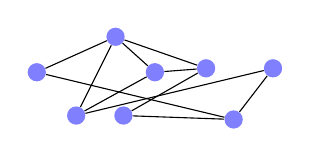
\begin{tikzpicture}
	[scale=.5,auto=left,every node/.style={circle,fill=blue!50, scale=0.7,-latex'}]
	\node (n2) at (0,0.4)  {};
	\node (n3) at (-2,-0.5)  {};
	\node (n5) at (2.3,-0.4)  {};
	\node (n1) at (1,-0.5) {};
	\node (n6) at (0.2,-1.6)  {};
	\node (n7) at (3,-1.7)  {};
	\node (n8) at (4,-0.4)  {};
	\node (n10) at (-1,-1.6)  {};
	\foreach \from/\to in {n5/n1,n1/n2,n2/n5,n2/n3,n10/n8, n10/n1, n2/n10, n7/n3, n7/n8, n6/n5, n7/n6}
	\draw (\from) -- (\to);
	\end{tikzpicture}
	\hspace{0.5cm}
	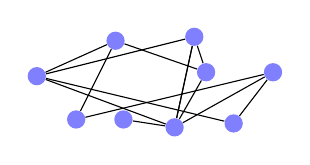
\begin{tikzpicture}
	[scale=.5,auto=left,every node/.style={circle,fill=blue!50, scale=0.7,-latex'}]
	\node (n2) at (0,0.4)  {};
	\node (n3) at (-2,-0.5)  {};
	\node (n4) at (1.5,-1.8) {};
	\node (n5) at (2.3,-0.4)  {};
	\node (n6) at (0.2,-1.6)  {};
	\node (n7) at (3,-1.7)  {};
	\node (n8) at (4,-0.4)  {};
	\node (n9) at (2,0.5)  {};
	\node (n10) at (-1,-1.6)  {};
	\foreach \from/\to in {n6/n4,n4/n5,n2/n5,n2/n3,n3/n4,n8/n4,n9/n4,n10/n8,n9/n5,  n3/n9, n4/n9, n2/n10, n7/n3, n7/n8}
	\draw (\from) -- (\to);
	\end{tikzpicture}
	
	\vspace{1cm}
	
	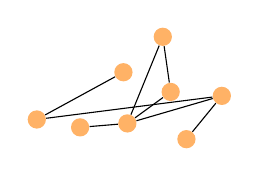
\begin{tikzpicture}
	[scale=.5,auto=left,every node/.style={circle,fill=orange!60, scale=0.7,-latex'}]
	\node (n4) at (1.2,-1.5) {};
	\node (n5) at (2.3,-0.7)  {};
	\node (n1) at (1.1,-0.2) {};
	\node (n6) at (0,-1.6)  {};
	\node (n7) at (2.7,-1.9)  {};
	\node (n8) at (3.6,-0.8)  {};
	\node (n9) at (2.1,0.7)  {};
	\node (n10) at (-1.1,-1.4)  {};
	\foreach \from/\to in {n6/n4,n4/n5,n8/n4,n10/n8,n9/n5, n10/n1, n4/n9,  n7/n8}
	\draw (\from) -- (\to);
	\end{tikzpicture}
	\hspace{0.5cm}
	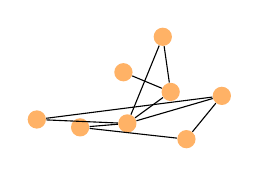
\begin{tikzpicture}
	[scale=.5,auto=left,every node/.style={circle,fill=orange!60, scale=0.7,-latex'}]
	\node (n4) at (1.2,-1.5) {};
	\node (n5) at (2.3,-0.7)  {};
	\node (n1) at (1.1,-0.2) {};
	\node (n6) at (0,-1.6)  {};
	\node (n7) at (2.7,-1.9)  {};
	\node (n8) at (3.6,-0.8)  {};
	\node (n9) at (2.1,0.7)  {};
	\node (n10) at (-1.1,-1.4)  {};
	\foreach \from/\to in {n6/n4,n4/n5,n5/n1,n8/n4,n9/n4,n10/n8,n9/n5, n7/n8, n6/n7, n10/n4}
	\draw (\from) -- (\to);
	\end{tikzpicture}
	
	
	\vspace{1cm}
	
	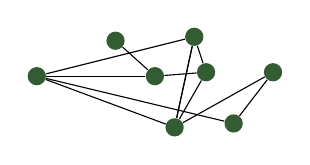
\begin{tikzpicture}
	[scale=.5,auto=left,every node/.style={circle,fill=black!80!green!80!, scale=0.7,-latex'}]
	\node (n2) at (0,0.4)  {};
	\node (n3) at (-2,-0.5)  {};
	\node (n4) at (1.5,-1.8) {};
	\node (n5) at (2.3,-0.4)  {};
	\node (n1) at (1,-0.5) {};
	\node (n7) at (3,-1.7)  {};
	\node (n8) at (4,-0.4)  {};
	\node (n9) at (2,0.5)  {};
	\foreach \from/\to in {n4/n5,n5/n1,n1/n2,n3/n4,n8/n4,n9/n4,n9/n5, n3/n9, n4/n9, n1/n3, n7/n3, n7/n8}
	\draw (\from) -- (\to);
	\end{tikzpicture}
	\hspace{0.5cm}
	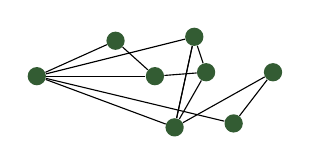
\begin{tikzpicture}
	[scale=.5,auto=left,every node/.style={circle,fill=black!80!green!80!, scale=0.7,-latex'}]
	\node (n2) at (0,0.4)  {};
	\node (n3) at (-2,-0.5)  {};
	\node (n4) at (1.5,-1.8) {};
	\node (n5) at (2.3,-0.4)  {};
	\node (n1) at (1,-0.5) {};
	\node (n7) at (3,-1.7)  {};
	\node (n8) at (4,-0.4)  {};
	\node (n9) at (2,0.5)  {};
	\foreach \from/\to in {n4/n5,n5/n1,n1/n2,n2/n3,n3/n4,n8/n4,n9/n4,n9/n5,  n3/n9, n4/n9,  n1/n3, n7/n3, n7/n8}
	\draw (\from) -- (\to);
	\end{tikzpicture}
\end{center}
\end{frame}


\begin{frame}
	\frametitle{Threat Model}
	\begin{center}
		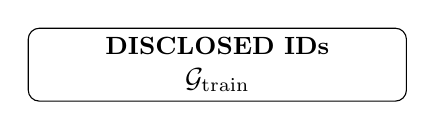
\begin{tikzpicture}
		\node[block] at (0,2) {{\small \textbf{DISCLOSED IDs}} \\ $\mathcal{G}_\text{train}$};
		\end{tikzpicture}
		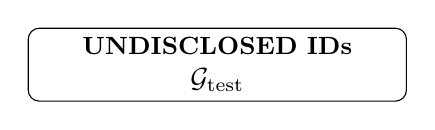
\begin{tikzpicture}
		\node[block] at (0,2) {{\small \textbf{UNDISCLOSED IDs}}\\ $\mathcal{G}_\text{test}$};
		\end{tikzpicture}
		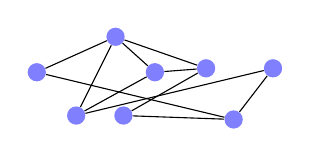
\begin{tikzpicture}
		[scale=.5,auto=left,every node/.style={circle,fill=blue!50, scale=0.7,-latex'}]
		\node (n2) at (0,0.4)  {};
		\node (n3) at (-2,-0.5)  {};
		\node (n5) at (2.3,-0.4)  {};
		\node (n1) at (1,-0.5) {};
		\node (n6) at (0.2,-1.6)  {};
		\node (n7) at (3,-1.7)  {};
		\node (n8) at (4,-0.4)  {};
		\node (n10) at (-1,-1.6)  {};
		\foreach \from/\to in {n5/n1,n1/n2,n2/n5,n2/n3,n10/n8, n10/n1, n2/n10, n7/n3, n7/n8, n6/n5, n7/n6}
		\draw (\from) -- (\to);
		\end{tikzpicture}
		\hspace{0.7cm}
		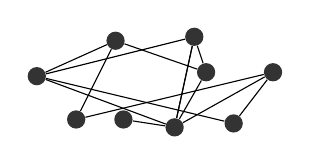
\begin{tikzpicture}
		[scale=.5,auto=left,every node/.style={circle,fill=black!80, scale=0.7,-latex'}]
		\node (n2) at (0,0.4)  {};
		\node (n3) at (-2,-0.5)  {};
		\node (n4) at (1.5,-1.8) {};
		\node (n5) at (2.3,-0.4)  {};
		\node (n6) at (0.2,-1.6)  {};
		\node (n7) at (3,-1.7)  {};
		\node (n8) at (4,-0.4)  {};
		\node (n9) at (2,0.5)  {};
		\node (n10) at (-1,-1.6)  {};
		\foreach \from/\to in {n6/n4,n4/n5,n2/n5,n2/n3,n3/n4,n8/n4,n9/n4,n10/n8,n9/n5,  n3/n9, n4/n9, n2/n10, n7/n3, n7/n8}
		\draw (\from) -- (\to);
		\end{tikzpicture}
		
		\vspace{0.1cm}
		
		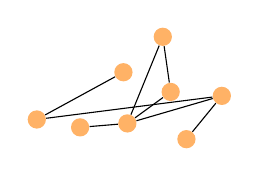
\begin{tikzpicture}
		[scale=.5,auto=left,every node/.style={circle,fill=orange!60, scale=0.7,-latex'}]
		\node (n4) at (1.2,-1.5) {};
		\node (n5) at (2.3,-0.7)  {};
		\node (n1) at (1.1,-0.2) {};
		\node (n6) at (0,-1.6)  {};
		\node (n7) at (2.7,-1.9)  {};
		\node (n8) at (3.6,-0.8)  {};
		\node (n9) at (2.1,0.7)  {};
		\node (n10) at (-1.1,-1.4)  {};
		\foreach \from/\to in {n6/n4,n4/n5,n8/n4,n10/n8,n9/n5, n10/n1, n4/n9,  n7/n8}
		\draw (\from) -- (\to);
		\end{tikzpicture}
		\hspace{0.5cm}
		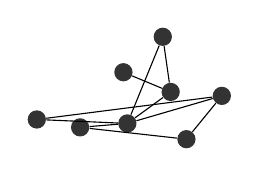
\begin{tikzpicture}
		[scale=.5,auto=left,every node/.style={circle,fill=black!80, scale=0.7,-latex'}]
		\node (n4) at (1.2,-1.5) {};
		\node (n5) at (2.3,-0.7)  {};
		\node (n1) at (1.1,-0.2) {};
		\node (n6) at (0,-1.6)  {};
		\node (n7) at (2.7,-1.9)  {};
		\node (n8) at (3.6,-0.8)  {};
		\node (n9) at (2.1,0.7)  {};
		\node (n10) at (-1.1,-1.4)  {};
		\foreach \from/\to in {n6/n4,n4/n5,n5/n1,n8/n4,n9/n4,n10/n8,n9/n5, n7/n8, n6/n7, n10/n4}
		\draw (\from) -- (\to);
		\end{tikzpicture}
		
		
		\vspace{0.1cm}
		
		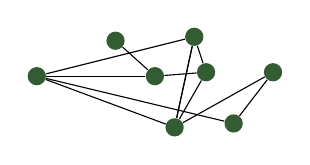
\begin{tikzpicture}
		[scale=.5,auto=left,every node/.style={circle,fill=black!80!green!80!, scale=0.7,-latex'}]
		\node (n2) at (0,0.4)  {};
		\node (n3) at (-2,-0.5)  {};
		\node (n4) at (1.5,-1.8) {};
		\node (n5) at (2.3,-0.4)  {};
		\node (n1) at (1,-0.5) {};
		\node (n7) at (3,-1.7)  {};
		\node (n8) at (4,-0.4)  {};
		\node (n9) at (2,0.5)  {};
		\foreach \from/\to in {n4/n5,n5/n1,n1/n2,n3/n4,n8/n4,n9/n4,n9/n5, n3/n9, n4/n9, n1/n3, n7/n3, n7/n8}
		\draw (\from) -- (\to);
		\end{tikzpicture}
		\hspace{0.5cm}
		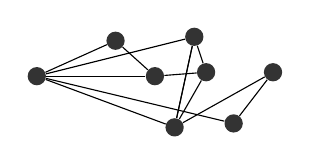
\begin{tikzpicture}
		[scale=.5,auto=left,every node/.style={circle,fill=black!80, scale=0.7,-latex'}]
		\node (n2) at (0,0.4)  {};
		\node (n3) at (-2,-0.5)  {};
		\node (n4) at (1.5,-1.8) {};
		\node (n5) at (2.3,-0.4)  {};
		\node (n1) at (1,-0.5) {};
		\node (n7) at (3,-1.7)  {};
		\node (n8) at (4,-0.4)  {};
		\node (n9) at (2,0.5)  {};
		\foreach \from/\to in {n4/n5,n5/n1,n1/n2,n2/n3,n3/n4,n8/n4,n9/n4,n9/n5,  n3/n9, n4/n9,  n1/n3, n7/n3, n7/n8}
		\draw (\from) -- (\to);
		\end{tikzpicture}
	\end{center}
	
	\begin{tikzpicture}[remember picture,overlay]
	\draw[line width=1pt] (6.,0.5) -- (6.,6.5);
	\end{tikzpicture}
Assumptions
\begin{itemize}
	\item  $\blacktriangleright$ closed-world
	\item  $\blacktriangleright$ partition point for each user randomly $\in (0.3, 0.7)$ of total obs. period
	\item  $\blacktriangleright$ state frequency information
\end{itemize}	
\end{frame}



\begin{frame}
	\frametitle{Threat Model}
	\begin{columns}
		\begin{column}{0.6\textwidth}
				\includegraphics[scale=0.5]{figs/network_setting.png}
		\end{column}
			\begin{column}{0.4\textwidth}
				\hspace{1cm}
		\includegraphics[width=3cm, height=3cm]{figs/adv1.png}
	\end{column}	
	\end{columns}
	%\centering
	%\includegraphics[width=5cm, height=7cm]{figs/tm1.png}
\end{frame}


\begin{frame}
	\frametitle{Attacks: Uninformed Adversary}
	\begin{columns}
		\begin{column}{0.2\textwidth}
			\begin{figure}
			\includegraphics[scale=0.25]{figs/unlabeled_networks.png}
			\end{figure}
		\end{column}
		\begin{column}{0.7\textwidth}
			\begin{center}
				\includegraphics[width=2.3cm, height=2.7cm]{figs/adv_uninformed.png}
				\begin{tikzpicture}
				\node[cloud, cloud puffs=15.7, minimum width=.3cm, minimum height=.3cm, inner sep=0pt,
				text width=4.2cm,draw] (cloud) at (-0.2,-0.2) {
					\begin{tabular}{}
					{\mbox{assign identities at random}} \\
				 {\mbox{\textbf{expected rank}}=$\mathbf{|\mathcal{L}|/2}$}
					\end{tabular}
				};
				\end{tikzpicture}
			\end{center}
		\end{column}	
	\end{columns}
\end{frame}

%$P\big(l_{G'}= l_{G_i}\big) = 1/|\mathcal{L}|, \\ \mbox{for every }  G_i \in \mathcal{G}_{\text{train}}$\\


\begin{frame}
	\frametitle{Attacks: Informed Adversary}
	\begin{columns}
		\begin{column}{0.2\textwidth}
			\includegraphics[scale=0.25]{figs/network_setting.png}
		\end{column}
		\begin{column}{0.8\textwidth}
\thinkA{
	\begin{tabular}{}
		 \mbox{assign \textbf{more probability mass}}\\
		 \mbox{to identities with \textbf{higher structural similarity}}
	\end{tabular}
}
\includegraphics[width=2.3cm, height=2.7cm]{figs/adv_informed.png}
		\end{column}	
	\end{columns}
	%\centering
	%\includegraphics[width=5cm, height=7cm]{figs/tm1.png}
\end{frame}


\begin{frame}
	\frametitle{Attacks: Informed Adversary}
	\begin{itemize}
		\item  $\blacktriangleright$ Posterior probability \\	
		\begin{tabular}{ ll }
		$P\big(l_{G'} =l_{G_i}$&$|\mathcal{G}_{\text{train}}, K\big) \propto  f\big(K(G_i, G')\big)$,\\ 
		& \text{for every}   $G_i \in \mathcal{G}_{\text{train}}$\\
		& \textcolor{red}{$K$ : graph similarity metric},\\ & $f$ : non-decreasing
		\end{tabular} 
		\item  $\blacktriangleright$ Privacy Loss 
		\begin{align*}
		\begin{split}
		PL\big(G';\mathcal{G}_{\text{train}}, K\big) = \frac{ P\big(l_{G'}= l_{G'_\text{true}}|\mathcal{G}_{\text{train}}, K\big)}{P\big(l_{G'}= l_{G'_\text{true}}\big)} -1
		\end{split}
		\end{align*}
	\end{itemize}
\end{frame}



\begin{frame}
	\frametitle{Graph Similarity Functions}
	\begin{block}{Graph Kernels} Express similarity as inner product of vectors with graph statistics \textcolor{black}{\Fontit{\citep{Vishwanathan2010}}}
		\begin{itemize}
			%\pause
			%\item  on \textbf{Graph Statistics} (e.g. weighted degree distribution)
			\pause
			\vspace{0.2cm}
			\item   $\blacktriangleright$ on \textbf{Atomic Substructures} (e.g. Shortest-Paths, Weisfeiler-Lehman subtrees) \\
			%\begin{center}
			%$K({G}, {G}')=\bigg   \langle \frac{\phi({G})}{||\phi({G})||}, \frac{\phi(G')}{||\phi(G')||} \bigg  \rangle$
			%\end{center}
			\pause
			\vspace{0.2cm}
			\item  $\blacktriangleright$ \textbf{Deep Kernels}: \Fontit{\citep{yanardagV15}} \\
			%\begin{center}
			%				$K(G, G') = \phi\big(G\big)^T \mathcal{M} \phi\big(G'\big)$
			%\end{center}
			 additionally learn an encoding similarities between substructures
		\end{itemize}
	\end{block}	
\end{frame}


\begin{frame}
	\centering
	\frametitle{Kernel-assisted Ranking}
	\begin{center}
		\begin{figure}
			\begin{subfigure}{\textwidth}
				\centering
				\includegraphics[width=.49\linewidth]{figs/kernels_evaluation}
			\end{subfigure}%
			\begin{subfigure}{\textwidth}
				\centering
				\includegraphics[width=.49\linewidth]{figs/rank_correct_}
			\end{subfigure}
			\label{fig:test}
		\end{figure}
	\end{center}
\vspace{0.01mm}
	\begin{itemize}
		\item mean correct rank under  \textbf{DSP} (random) at $\mathbf{140}$ ($750$)
	\end{itemize}
\end{frame}

\begin{frame}
	\frametitle{Privacy Loss}
	\begin{columns}
		\begin{column}{0.55\textwidth}
			\includegraphics[width=7cm, height=6cm]{figs/posterior_privloss_.pdf}
		\end{column}
		\begin{column}{0.45\textwidth}
			\vspace{1cm}
			\begin{itemize}
				\item $f(\cdot)=\frac{1}{rank(\cdot)}$
				\item median $ = 2.52 $
			\end{itemize}
		 \visible<.(1)>{\includegraphics[width=3cm, height=3cm]{figs/adv_celebrating}}
		\end{column}
	\end{columns}
\end{frame}


\begin{frame}
	\frametitle{Takeaways}
	
	\begin{itemize}
		\item  $\blacktriangleright$ \textbf{Location pruning} does not necessarily make network more privacy-preserving
		\vspace{0.1cm}
		\item  $\blacktriangleright$ Including \textbf{rare transitions} in longitudinal mobility did \textbf{not} add discriminative
information
		\vspace{0.1cm}
		\item  $\blacktriangleright$ Deanonymization is assisted by \textbf{frequency of
locations}, \textbf{directionality of transitions}
	\end{itemize}
\end{frame}



\begin{frame}
	\frametitle{Summary of findings}
	\begin{block}{}%{We investigated privacy properties of \textbf{graph
	%			representations} of longitudinal mobility}
		%\begin{itemize}
		%	\item New deanonymization attack on mobility data using
		%	\textbf{structural similarity} with historical information
		%	\item Evaluation on \textbf{large dataset of cell-tower location traces}
				\begin{itemize}
				\item $\blacktriangleright$ graph representations of mobility display \textbf{distinct structure},
				\textbf{even for small number of nodes}
				\item  $\blacktriangleright$ \textbf{$ \mathbf{< 20}$ locations} are enough to identify uniquely a
				population of \mbox{\textbf{$ \mathbf{1500} $ users}}
				\item  $\blacktriangleright$ \textbf{kernel-based distance functions} can quantify similarity in absence
				of location semantics and fine-grained temporal information
				\item  $\blacktriangleright$ probabilistic deanonymization using similarity with historical
				data can achieve \textbf{median success probability $ \mathbf{3.5\times} $ higher
					than a random mechanism}
			\end{itemize}
			
		%\end{itemize}
	\end{block}
\end{frame}



\begin{frame}
	\frametitle{Future Directions}
	\begin{itemize}
		\item  $\blacktriangleright$ \textbf{Geometry of kernel feature spaces}: high dimensional space with meaningful neighborhood relations 
		\item  $\blacktriangleright$ \textbf{Other graph similarity techniques}: network alignment,
		persistent cascades, frequent/discriminative substructure mining, anonymous walks, spectral representations
		\item  $\blacktriangleright$ Application to \textbf{other categories of sequential datasets}: web browsing
		behaviour, smartphone app usage
		\item  $\blacktriangleright$ \textbf{Formal privacy guarantees} for mobility networks
		\item  $\blacktriangleright$ \textbf{Utility preserving defense mechanisms}: kernel-agnostic defense, randomisation of node
		\item  $\blacktriangleright$ \textbf{Generative mechanisms} for synthetic traces with anonymity guarantees
		attributes, perturbations of edges, node removal
	\end{itemize}
\end{frame}



\begin{frame}
	\LARGE{\textbf{II. Bayesian Pseudocoresets}}
\end{frame}


\begin{frame}
	\LARGE{\textbf{III. $\beta$-Cores: Robust Large-Scale Bayesian Data Summarization in the Presence of Outliers}}
\end{frame}



\begin{frame}
	\begin{center}
		\centering
		\Fontvilarge
		\textcolor{red}{Thanks!} \\
		\vspace{0.15cm}
		Any Questions? \\ 
		\vspace{0.15cm}
		\includegraphics[width=3.5cm,height=3.5cm]{qr.png} \\ 
		\vspace{0.25cm}
		dm754@cam.ac.uk
	\end{center}
	%\blfootnote{We would like to acknowledge the support of the Alan Turing Institute and Nokia Bell Labs}
\end{frame}


\begin{frame}[allowframebreaks]{References}
	\tiny %\scriptsize
	\bibliography{references.bib}
\end{frame}

\end{document}
